\chapter{Introducción}\label{ch:introduccion}

Este proyecto está publicado bajo la licencia GNU General Public License v3~\cite{gplv3}.
Se puede acceder a través de GitHub por medio de estos enlaces: \href{https://github.com/Marodseg/confianza-animal-backend}{API}
y \href{https://github.com/Marodseg/confianza-animal-frontend}{página web}.


\section{Motivación y contexto}\label{sec:motivacion-y-contexto}

La adopción animal es una de las mejores opciones para combatir el gran problema con el que se enfrenta
abandono animal. Sin embargo, en la actualidad, las asociaciones que se dedican a llevar a cabo esta tarea,
cuentan con múltiples dificultades para gestionar toda la información de los animales
que acogen y buscan dar en adopción. El elevado número de mascotas abandonadas a diario, hace que
las organizaciones no puedan ofrecer una atención personalizada a cada una de ellas. Además, la falta de medios
de comunicación y difusión hace que muchas de las mascotas que buscan un nuevo hogar no
puedan ser adoptadas. A todo esto hay que sumarle la falta de voluntarios que puedan contribuir en esta labor y
la falta de recursos económicos que les permitan tener las herramientas necesarias para facilitar y agilizar
todas las gestiones que conlleva mantener a un animal hasta que encuentre un nuevo hogar. \\

Estos motivos han llevado a la creación de este proyecto que, de alguna forma, pretende ayudar a este sector
por medio de la tecnología. Consiste en la creación de una \textbf{API} (\textit{Application Web Interface}) así como de una aplicación web que por medio de
los servicios proporcionados por la \textbf{API}, permita facilitar a las organizaciones y protectoras la gestión de los
animales que acogen, con información detallada de cada uno de ellos, como su edad, raza, estado de salud, entre otros.
Además, la aplicación web permitirá a las organizaciones difundir toda la información necesaria para que sus animales
puedan ser vistos por personas interesadas en su adopción llevando a cabo un seguimiento del proceso. \\


\section{Descripción del problema}\label{sec:descripcion-del-problema}

Datos de la prestigiosa revista \href{https://www.nationalgeographic.es/animales/2021/12/espana-lider-europea-en-abandono-de-animales-700-cada-dia}{National Geographic} o
la conocida \href{https://www.fundacion-affinity.org}{Fundación Affinity} aseguran que España lidera desde años el
ranking europeo de abandono de animales con una media de 700 animales al día. La falta de concienciación en la sociedad y
de recursos económicos en las protectoras y asociaciones, acompañados por la dejadez política, son las principales causas de este problema. \\

\begin{figure}[H]
\centering
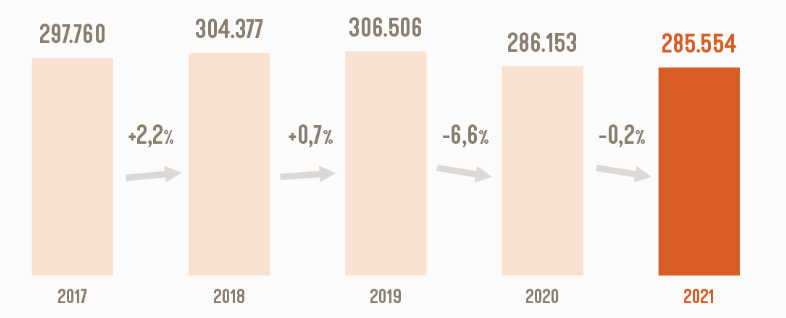
\includegraphics[width=0.5\textwidth]{imgs/grafica_abandonos.png}
    \caption{Gráfica de abandonos de animales en España en los últimos años. Fuente~\cite{affinity}}
    \label{fig:grafica_abandonos}
\end{figure}

Si bien es cierto que podemos observar en la gráfica que el número de animales abandonados ha disminuido en los últimos años, la situación no es tan
alentadora como parece. Los voluntarios de las protectoras y asociaciones de animales han tenido que hacer frente a la
situación de forma altruista para mantener el funcionamiento de las mismas, así como para atender a los animales que
llegan a sus instalaciones.

El paso del COVID ha agravado la situación, ya que muchas personas han tenido que abandonar a sus mascotas por no poder
prestarles atención y cuidarlas. El número de animales acogidos en los últimos años ha disminuido considerablemente, hasta el punto en el que
se ha establecido una etapa llamada generación COVID. \\

Es importante destacar que este problema no yace en la falta de voluntarios o iniciativas, sino en la falta de
concienciación y responsabilidad de la sociedad. Es necesario un compromiso de ciudadanos y autoridades para
apoyar y financiar a todos aquellos que realizan un esfuerzo de forma altruista para mejorar la situación de los
animales. \\

Actualmente, las protectoras y organizaciones se encuentran en una situación delicada y de saturación que genera un problema de
gestión en la información de los animales que acogen y buscan dar un nuevo hogar. A esto, se suma un
sector tecnológico que no ha prestado atención a este problema, ya que no le es rentable y no se encuentra
en su línea de negocio. \\


\section{Objetivos}\label{sec:objetivos}

Durante el desarrollo de este proyecto se han establecido una serie de objetivos que se deben cumplir de forma
progresiva. Estos objetivos se han establecido en función del tiempo de la asignatura, de las herramientas y los
conocimientos que se disponen y de las principales necesidades de las asociaciones y protectoras de animales: \\

\begin{enumerate}
    \item El principal objetivo es crear una \textbf{API} para la gestión de animales en adopción. Dentro de este gran objetivo,
    se puede hacer una subdivisión en los siguientes puntos a cumplir:
    \begin{itemize}
        \item Garantizar la seguridad de la información que circula entre la web, \textbf{API} y base de datos.
        \item Permitir a las organizaciones una gestión de la información de forma clara y sencilla.
        \item Permitir a los usuarios la adopción de un animal así como conocer el progreso y estado de las solicitudes.
        \item Permitir establecer un flujo de comunicación entre las organizaciones y los usuarios durante el proceso de adopción.
    \end{itemize}
    \item Crear una página web enfocada exclusivamente a las organizaciones que permita comprobar el correcto funcionamiento de la \textbf{API}.
    El diseño debe permitir una navegación clara y sencilla así como una gestión de la información rápida y eficiente.
    \item Aprender nuevos paradigmas de desarrollo de software y nuevas tecnologías.
    \item Identificar posibles mejoras y ampliaciones para el proyecto en futuros trabajos.
\end{enumerate}


\section{Metodología y herramientas}\label{sec:metodologia-y-herramientas-de-seguimiento}

Una vez definidos los objetivos del problema a resolver, en este apartado se explica la metodología y herramientas
utilizadas durante el desarrollo del proyecto.

\subsection{Metodología}\label{subsec:metodologia}

Para conseguir los objetivos propuestos, se ha seguido una metodología ágil en la que se ha diferenciado de forma
clara entre la creación de la \textbf{API}, la creación de la web y la propia documentación del proyecto. \\

La elección de la metodología ágil se debe a que permite adaptarse de forma rápida a cualquier cambio que pueda
surgir durante el desarrollo del proyecto y que además se basa en un trabajo incremental y continuo. Esto permite
que el proyecto se pueda llevar a cabo en un tiempo limitado, con una serie de tareas que se agrupan en
diferentes fases y que conforme se van completando de forma progresiva van añadiendo valor al producto final. \\

\begin{figure}[H]
\centering
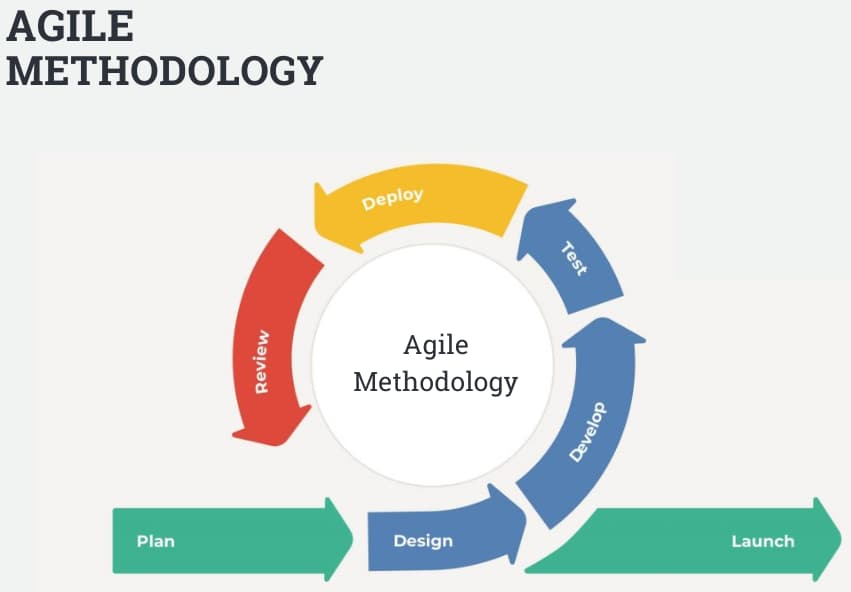
\includegraphics[width=0.5\textwidth]{imgs/metodologia_agil.jpg}
    \caption{Diagrama de la metodología ágil}
    \label{fig:metodologia_agil}
    \caption*{Fuente: \href{https://interqualitybg.com/en/resources/scrum-and-agile-resources/agile-methodology}{Interquality}}
\end{figure}

La metodología ágil que se ha utilizado en este proyecto es \textbf{Scrum}, ya que es una de las más populares en el
desarrollo de software actual, permite de una manera sencilla y ordenada llevar a cabo el desarrollo de un proyecto y
ofrece una gran flexibilidad a la hora de gestionar los cambios que puedan surgir en el proceso. \\

Si bien es verdad que el uso de estas técnicas se llevan a cabo en equipos con más integrantes y cuentan con
diferentes fases que priorizan la comunicación y colaboración en equipo, se ha decidido adaptar para que se pueda
llevar a cabo de forma individual sin dejar atrás los fundamentos y pilares de estas metodologías:

\begin{itemize}
    \item División del proyecto en diferentes fases compuestas por tareas (sprints).
    \item Contabilización de las horas invertidas en cada tarea y en el proyecto en general (medición del progreso).
    \item Fácil adaptación a posibles cambios.
    \item Trabajo incremental y continuo.
\end{itemize}

\subsection{Herramientas de seguimiento}\label{subsec:herramientas-de-seguimiento}

Para llevar a cabo los objetivos marcados por la metodología ágil, se han utilizado diferentes herramientas que
han permitido llevar un seguimiento del progreso del proyecto y de las tareas que se han ido completando
de una forma sencilla y ordenada. \\

Como gestión de control de versiones se ha utilizado \textbf{Git}. Esta herramienta permite el seguimiento de
cambios en el código así como la colaboración de diferentes personas que trabajen o quisieran colaborar en el
proyecto. Además, Git funciona de forma local y permite trabajar de forma offline, dando la posibilidad de
trabajar en cualquier momento y a cualquier hora. \\

Para alojar los proyectos, tanto de la \textbf{API} como de la web, se ha utilizado \textbf{GitHub}. Esta tecnología que
a diferencia de Git necesita de una conexión a internet para poder trabajar, permite el seguimiento y revisiones del
código, colaboración con otros usuarios y múltiples herramientas integradas que facilitan el desarrollo de software de
las cuales se han utilizado las siguientes:

\begin{itemize}
    \item \textbf{GitHub Actions}: permite la automatización de tareas y la integración continua.
    \item \textbf{GitHub Projects}: permite la creación de tableros de tareas y la gestión de los sprints.
    \item \textbf{GitHub Secrets}: permite la gestión de las variables de entorno de forma segura.
\end{itemize}

En los siguientes apartados se profundiza en cada una de estas herramientas y se explican sus usos en el proyecto.

\subsubsection{Historias de usuario (HU)}
GitHub permite la creación de tareas que pueden diferenciarse entre sí por medio de etiquetas clasificatorias o
por medio de una nomenclatura que permita identificarlas de forma rápida como por ejemplo \textbf{HU-1} para
la primera historia de usuario. \\

Las etiquetas que se han utilizado para diferenciar las tareas son las siguientes:

\begin{itemize}
    \item \textbf{task}: para señalar que se trata de una tarea.
    \item \textbf{bug}: para señalar que se trata de un error.
    \item \textbf{documentation}: para señalar que se trata de una tarea de documentación.
    \item \textbf{WIP}: para señalar que se trata de una tarea en progreso (Work In Progress).
    \item \textbf{HU}: para señalar que se trata de una historia de usuario.
    \item \textbf{don't merge}: para señalar que se trata de una tarea que no se debe mezclar con el resto del proyecto.
\end{itemize}

Una vez aclarado el uso de las etiquetas, se procede a explicar las diferentes historias de usuario que se han
desarrollado en el proyecto y que han tratado reflejar las necesidades de los usuarios y las organizaciones:

\begin{itemize}
    \item \textbf{HU-1: Como lector quiero poder conocer las bases del proyecto de manera clara y ordenada a partir de
    la memoria proporcionada}: esta historia de usuario es la asociada a la creación de la documentación del proyecto.
    \item \textbf{HU-2: Como organización quiero poder gestionar mis animales en adopción de manera sencilla}: esta
    historia de usuario cuenta con los siguientes criterios de aceptación:
        \begin{enumerate}
            \item Visualizar todos mis animales (perros/gatos)
            \item Añadir un nuevo animal
            \item Subir imágenes de los animales
            \item Borrar imágenes de los animales (antiguas, borrosas, etc.)
            \item Editar el perfil y los datos de mis animales
            \item Borrar animales que no estén disponibles para la adopción
            \item Visualizar las peticiones de mis animales por parte de los usuarios
            \item Aceptar o rechazar las peticiones de adopción de mis animales realizadas por los usuarios
        \end{enumerate}
    que han de ser cumplidos para que la historia de usuario se considere completada.
    \item \textbf{HU-3: Como organización quiero poder gestionar mi información personal}: esta historia de usuario cuenta
    con los siguientes criterios de aceptación:
        \begin{enumerate}
            \item Visualizar mi perfil
            \item Editar la información de mi perfil
            \item Subir imágenes a mi perfil
        \end{enumerate}
    que han de ser cumplidos para que la historia de usuario se considere completada.
    \item \textbf{HU-4: Como usuario quiero poder adoptar un animal}: esta historia de usuario cuenta con los siguientes
    criterios de aceptación:
        \begin{enumerate}
            \item Visualizar todos los animales disponibles para la adopción
            \item Visualizar los detalles de un animal dentro de una organización concreta
            \item Filtrar la búsqueda de animales con parámetros como raza, tamaño, sexo, etc.
            \item Solicitar la adopción de un animal
        \end{enumerate}
    que han de ser cumplidos para que la historia de usuario se considere completada.
    \item \textbf{HU-5: Como usuario quiero poder gestionar mi información personal}: esta historia de usuario cuenta
    con los siguientes criterios de aceptación:
        \begin{enumerate}
            \item Visualizar mi perfil
            \item Editar la información de mi perfil
            \item Subir imágenes a mi perfil
        \end{enumerate}
    que han de ser cumplidos para que la historia de usuario se considere completada.
\end{itemize}

Algunas de estas tareas y sus historias de usuario se pueden ver en la siguiente imagen:

\begin{figure}[H]
    \centering
    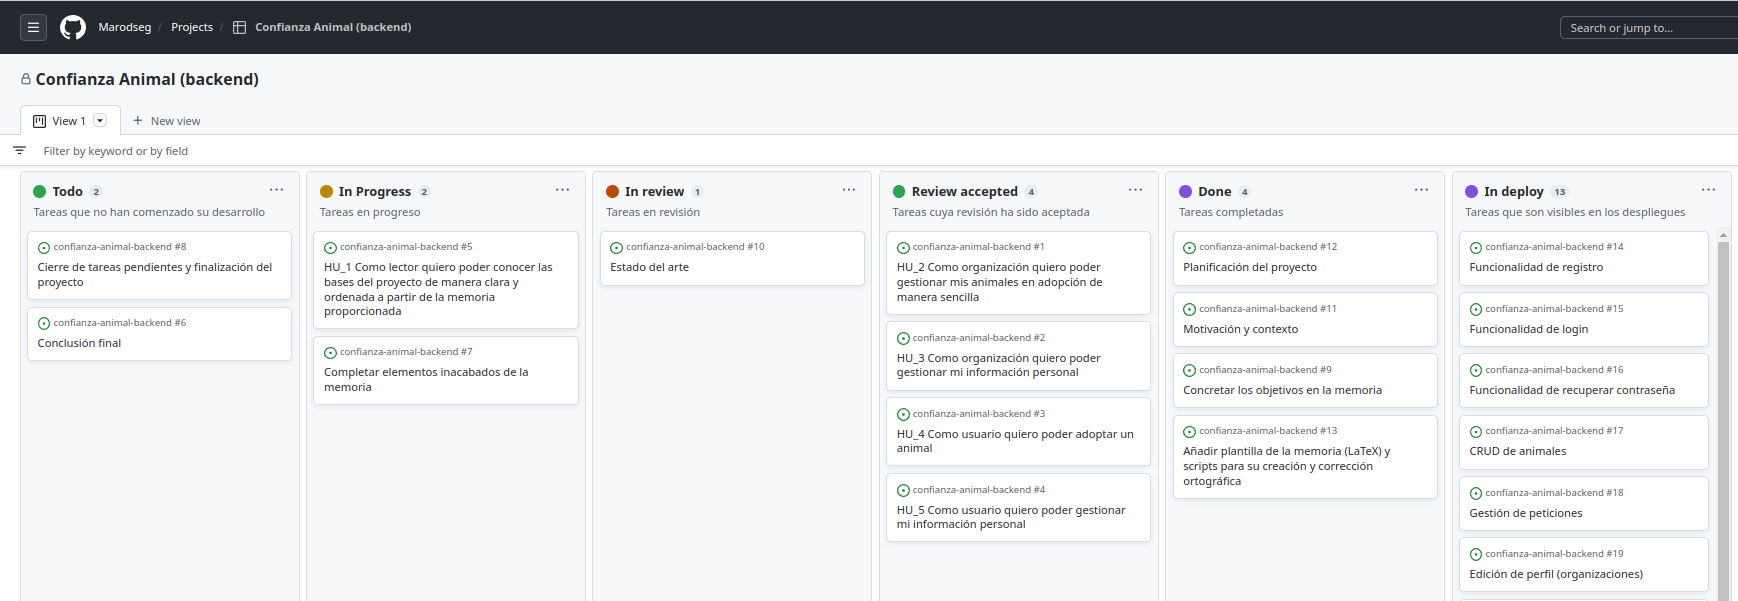
\includegraphics[width=0.9\textwidth]{imgs/tablero-github.png}
    \caption{Tablero de GitHub para el seguimiento de tareas}
    \label{fig:tablero-github}
\end{figure}

\subsubsection{Milestones}

El desarrollo del proyecto se ha dividido en \textit{milestones} (o hitos) que son entregables que marcan
el progreso del proyecto hacia la versión final. Son importantes para mantener un objetivo claro y tener una
forma de medir el éxito del producto a desarrollar. Los \textit{milestones} que se han llevado a cabo son los
siguientes:

\begin{enumerate}
    \item \textbf{Base e introducción}: engloba toda la preparación inicial del proyecto así como del entorno de
    trabajo. Además incluye los primeros pasos en la documentación, teniendo la historia de usuario \textbf{HU-1}
    mencionada anteriormente como objetivo principal de este hito.
    \item \textbf{Gestión de animales en adopción}: en este hito se recogen todos los objetivos relacionados con
    la administración de animales en una entidad de adopción (organización, perrera, asociación, etc.) y los
    usuarios que deseen adoptar alguno de ellos. Esto incluye
    la implementación de servicios que permitan a estas entidades gestionar sus animales, así como llevar un control
    de las peticiones de los usuarios por los mismos. Y servicios que permitan a los usuarios
    visualizar los animales y tener la posibilidad de notificar a la entidad su interés por alguno de ellos.
    \item \textbf{Conclusión}: en este hito se recogen todos los objetivos relacionados con la finalización del
    proyecto, incluyendo el cierre de tareas pendientes, finalización de la documentación y la entrega del proyecto.
\end{enumerate}

\begin{figure}[H]
    \centering
    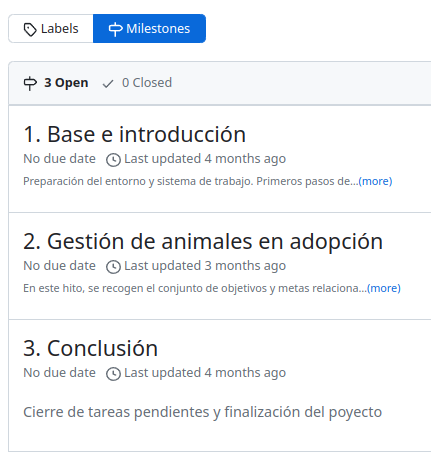
\includegraphics[width=0.5\textwidth]{imgs/milestones.png}
    \caption{Milestones del proyecto}
    \label{fig:milestones}
\end{figure}


\subsubsection{Integración continua}

La integración continua es una práctica llevada a cabo en el desarrollo de software que consiste en la ejecución
automática de pruebas y tareas de compilación cada vez que se realiza un cambio en el código fuente. De esta
forma se pueden detectar errores y permite corregirlos antes de que se produzca un fallo en el sistema. \\

Para llevar a cabo la integración continua se ha utilizado \textit{GitHub Actions}, un servicio que ofrece
GitHub para automatizar tareas en el repositorio. En este caso se ha utilizado para ejecutar diferentes pruebas
de calidad y testing de código así como el despliegue de la aplicación y la \textbf{API}:


\begin{itemize}
    \item \textbf{Estilo de código}: se ha utilizado \textit{Black} para comprobar el estilo de código de la
    \textbf{API} y \textit{Lint y Prettier} para la web. Estos servicios se ejecutan cada vez que se realiza un
    \textit{push} en cada repositorio y no permiten que se mezcle un código que no completa las pruebas con éxito.

    \newpage

    Se puede ver un ejemplo de la ejecución de estos servicios en las siguientes imágenes: \\

    \begin{figure}[H]
        \centering
        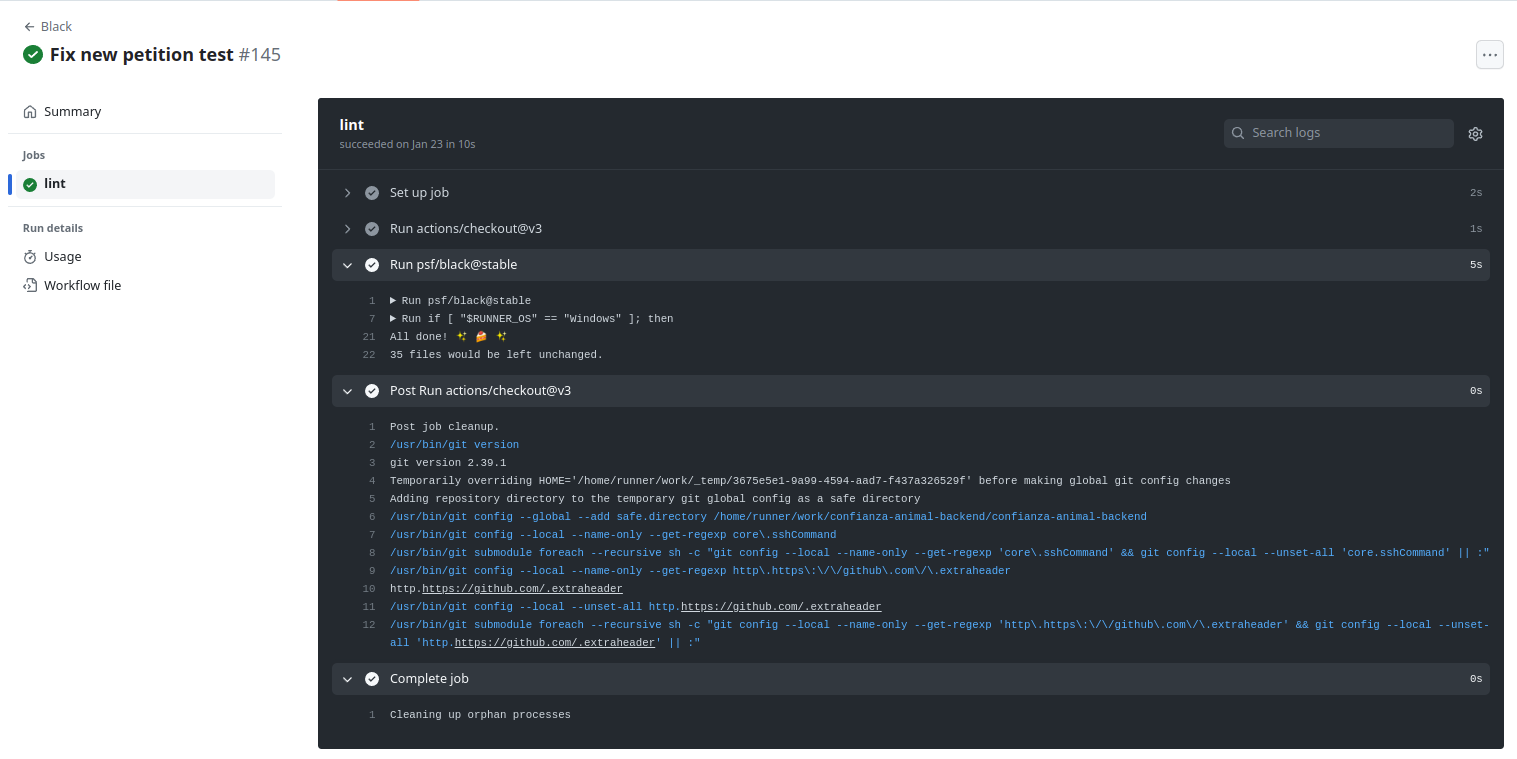
\includegraphics[width=0.9\textwidth]{imgs/black-action.png}
        \caption{GitHub Action Black en API}
        \label{fig:black-action}
    \end{figure}

    \begin{figure}[H]
        \centering
        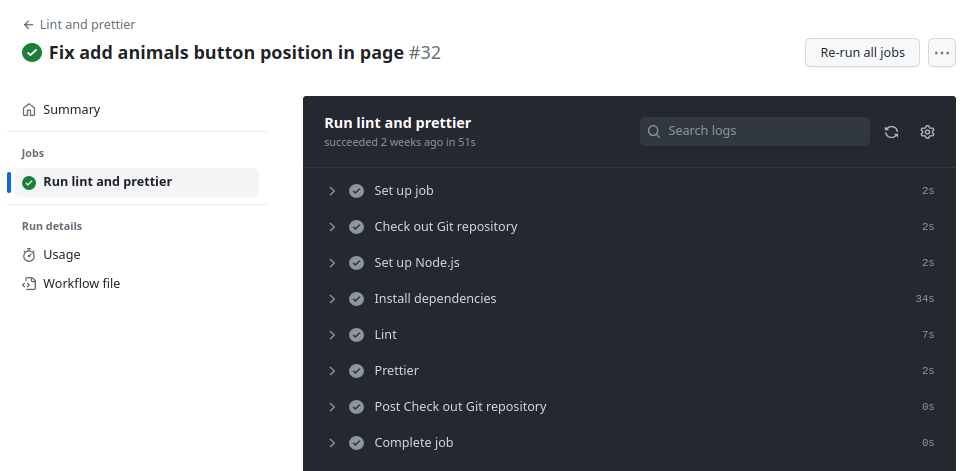
\includegraphics[width=0.9\textwidth]{imgs/lint-prettier-action.png}
        \caption{GitHub Action Lint y Prettier en Web}
        \label{fig:lint-prettier-action}
    \end{figure}

    \newpage

    \item \textbf{Testing}: se ha utilizado \textit{Pytest} para realizar las pruebas de la \textbf{API} y \textit{Karma} y
    \textit{Jasmine} para las pruebas de la web. Estos servicios se ejecutan cada vez que se realiza un
    \textit{push} en cada repositorio y no permiten que se mezcle el código con el resto si alguna de las pruebas falla.
    \item \textbf{Documentación}: para garantizar la calidad en la generación de este documento se ha utilizado un
    servicio que revisa la ortografía de cada cambio que se propone en el documento.
    \item \textbf{Despliegues}: se ha utilizado \textit{Render} para el despliegue de la API y \textit{Firebase Hosting} para
    el despliegue de la web. Estos servicios se ejecutan cada vez que se realiza un \textit{push} en cada repositorio
    sobre la rama principal y permiten el despliegue en un entorno de producción. En ambos repositorios se realiza
    una comprobación previa de que el código cumple con todas las pruebas mencionadas anteriormente para garantizar
    que los despliegues se realizan con éxito.
\end{itemize}

